\chapter{This is Chapter2}

\lipsum[1]%generic text

\section{This is a section}
Now I will use my acronym: the \gls{ecb} is the central bank of Europe. Actual president of the \gls{ecb} is Christine Largarde.

The \gls{eu} is a union of 27 European member states. In 2012 the \gls{eu} received the Nobel Peace Prize.

\subsection{This is a subsection}
G.A. Akerlof wrote one of the most popular papers in economics which is called the Market for "Lemons"\parencite{akerlof1970}.
\begin{figure}[H] %H=Forced Here; h=here(could be changed because of formatting; t=top; b=bottom of the page
    \centering
    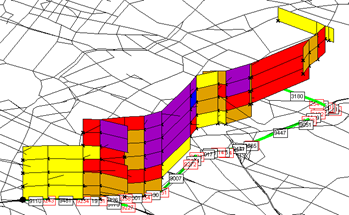
\includegraphics[height=50mm]{Images/TestPic.png} %choose your uploaded image from folder "Images"
    \caption{Test Figure2} %figure caption
    \label{fig:TestFigure2} %labelling for internal reference
\end{figure} 

Romer \parencite{romer1990endogenous}

\subsubsection{This is a subsubsection}
This is one level below subsection

\paragraph{This is a paragraph}
This is one level below subsubsection


\subparagraph{This is a subparagraph}
This is one level below paragraph

\begin{center}
\begin{table}[h]%H=Forced Here; h=here(could be changed because of formatting; t=top; b=bottom of the page
\centering
\begin{tabular}{lll}%l=left c=center r=right; "|" for vertical line
	\hline %insert line
	\textbf{left column} & \textbf{mid column} & \textbf{right column} \\
	\hline
	A & B & C \\
	! & 2 & 3 \\
	a & b & c \\
	i & ii & iii \\
	\hline
\end{tabular}
\caption{Test table2}
\label{tab:threecols2}
\end{table}
\end{center}
    


